\chapter{Resultados Obtidos}
\label{chapter:validation}

\begin{introduction}
Este capítulo apresenta os resultados experimentais obtidos com o protótipo da mesa sísmica, avalia o desempenho do modo de operação implementado e expõe, com detalhe, as razões mecânicas que impedem a reprodução fiel do registo sísmico de El Centro.
\end{introduction}

\section{Protótipo Desenvolvido}
\label{sec:prototipo}

O protótipo da mesa sísmica bi-axial foi concluído e testado em laboratório. A Figura~\ref{fig:prototipo-completo} mostra o conjunto montado, incluindo a base fixa, a plataforma móvel superior, as quatro colunas com rótulas e os quatro motores NEMA17 com os respetivos fusos trapezoidais.

% TODO: Inserir figura do protótipo completo montado.
\begin{figure}[h]
  \centering
  \begin{subfigure}{0.48\textwidth}
    \centering
    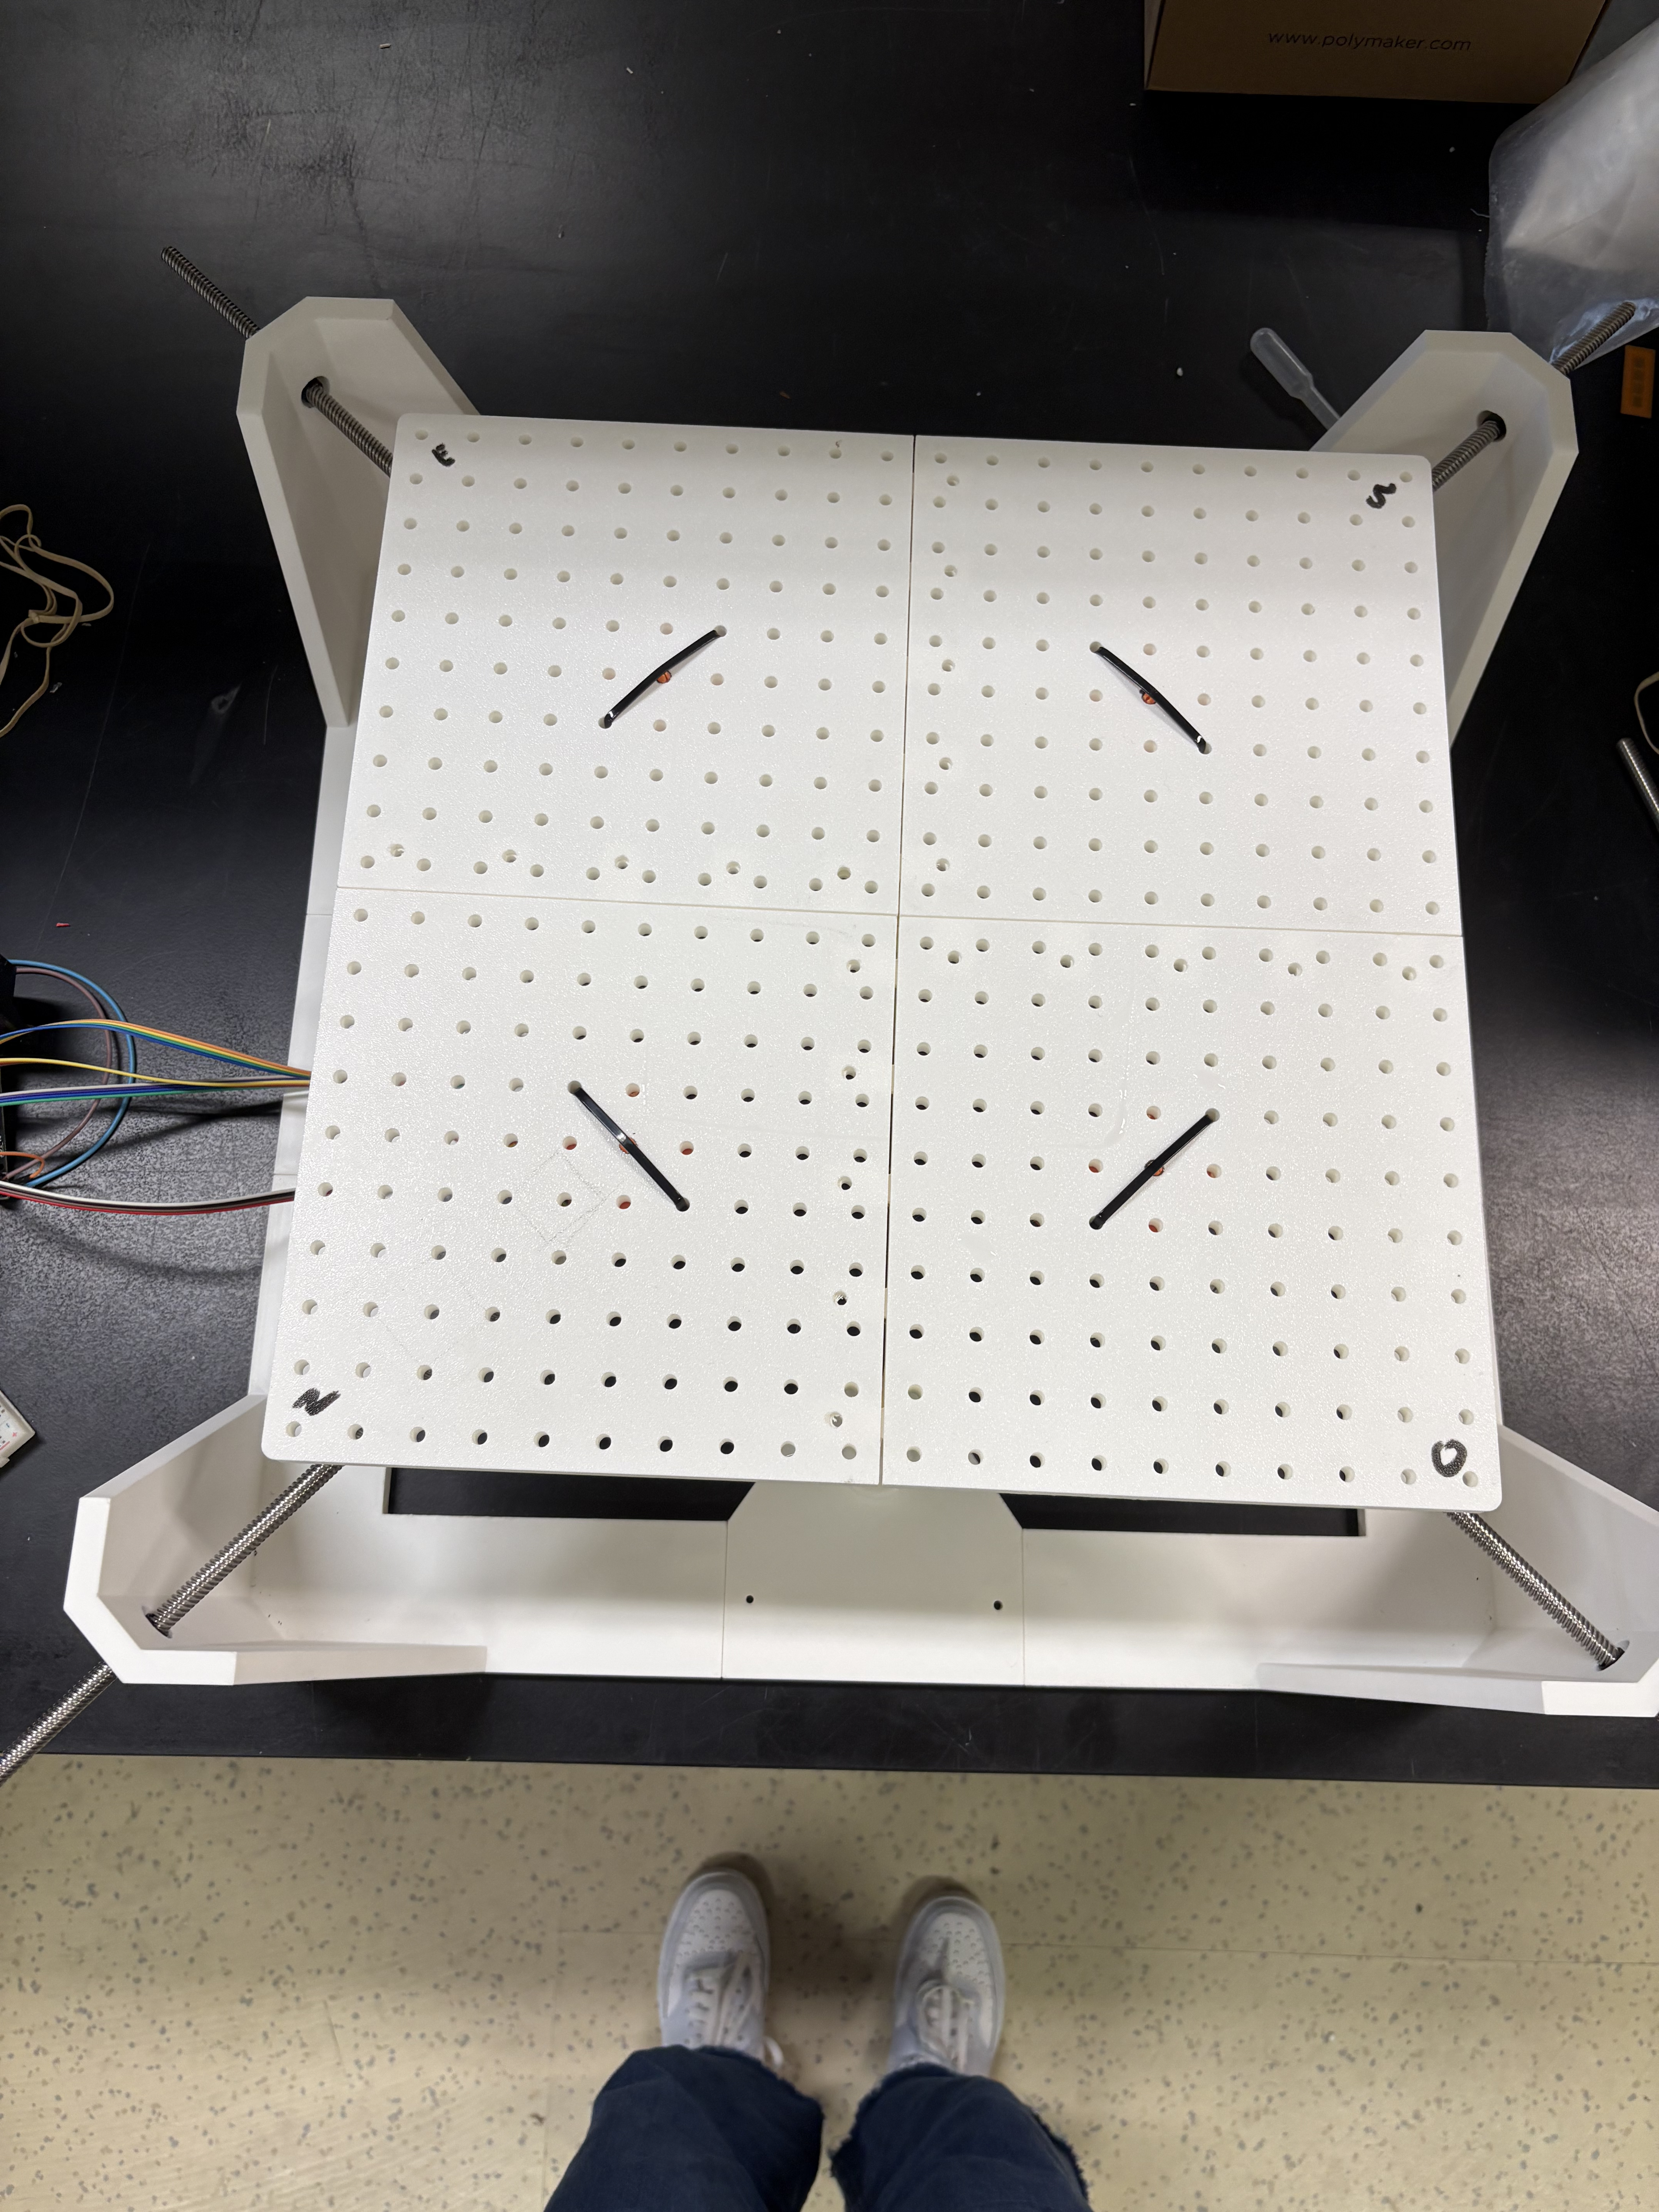
\includegraphics[trim=0cm 35.0cm 0cm 0cm, clip, width=.8\linewidth]{figs/prototipo_s.png}
    \caption{Visão Superior}
    \label{fig:prototipo-superior}
  \end{subfigure}
  \hfill % Espaçamento horizontal entre as imagens
  \begin{subfigure}{0.48\textwidth}
    \centering
    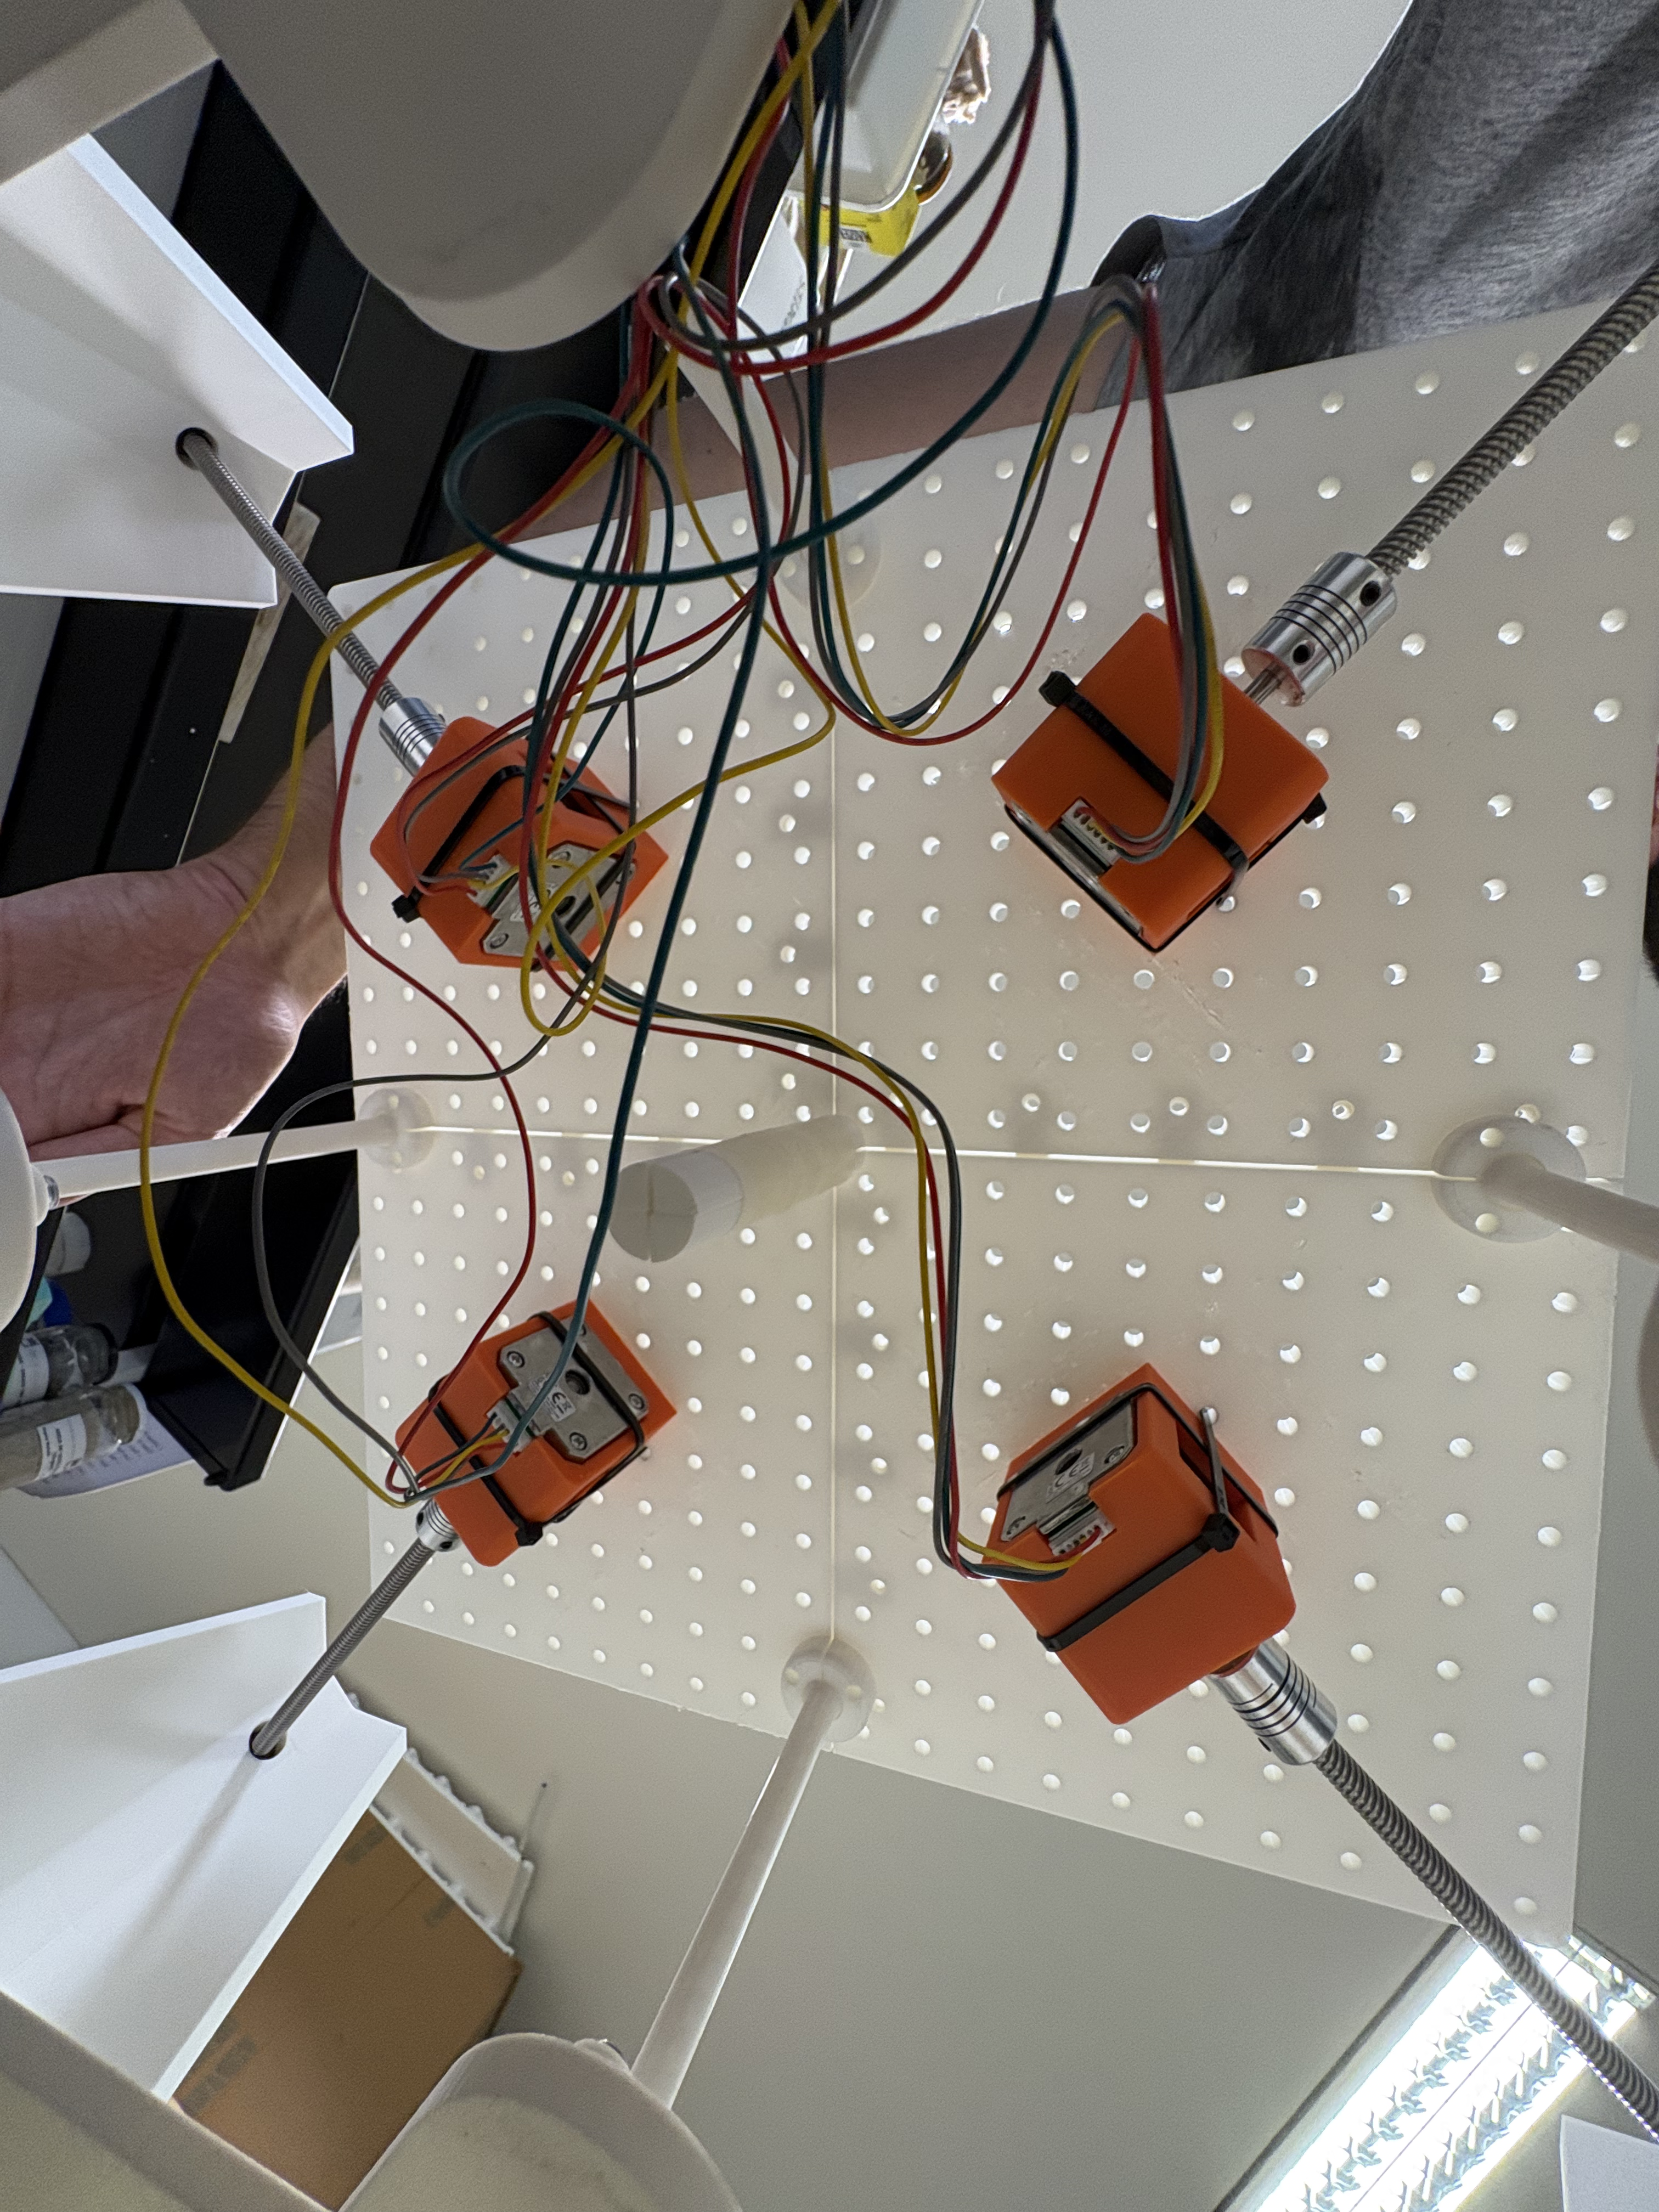
\includegraphics[trim=0cm 13.0cm 0cm 13cm, clip, width=.8\linewidth]{figs/prototipo_i.png}
    \caption{Visão Inferior}
    \label{fig:prototipo-inferior}
  \end{subfigure}
  
  \caption{Protótipo da mesa sísmica bi-axial montado em laboratório.}
  \label{fig:prototipo-completo}
\end{figure}

\section{Validação do Modo de Frequência Variável com Web UI}
\label{sec:validacao-web}

O modo de operação principal - movimento sinusoidal bi-axial com parâmetros configuráveis via interface web - foi validado experimentalmente com sucesso. Os ensaios realizados confirmaram o seguinte:

\begin{itemize}
    \item \textbf{Movimento bi-axial simultâneo:} A plataforma executa deslocamentos nos eixos NS e EW em simultâneo, com os quatro motores a trabalhar de forma sincronizada.
    \item \textbf{Percurso elíptico/circular:} A desfasagem de 90° entre os eixos NS e EW produz um percurso elíptico da plataforma, observável a olho nu. Quando a amplitude é igual nos dois eixos, o percurso é aproximadamente circular.
    \item \textbf{Interface web funcional:} Os parâmetros de frequência, amplitude e intervalo foram alterados em tempo real via browser, sem qualquer reconexão USB ou interrupção do movimento. A interface \texttt{http://192.168.4.1} foi acedida com sucesso por smartphone e computador portátil, confirmando a funcionalidade do modo Access Point.
    \item \textbf{Confirmação de aceleração:} Um ensaio circular a baixa frequência com uma aplicação sismógrafo de smartphone colocada sobre a plataforma registou acelerações de ordem de grandeza comparável a um sismo de baixa intensidade ($\approx$4 na escala de Richter), confirmando que a plataforma imprime aceleração mensurável ao modelo.
\end{itemize}

\textbf{Conclusão:} o modo de frequência variável cumpre os requisitos funcionais RF1 (movimento bi-axial), RF2 (frequência variável) e RF-Web (interface web embarcada), definidos no Capítulo~\ref{chapter:architecture}.


\section{Análise das Limitações Mecânicas para Reprodução Sísmica Real}
\label{sec:limitacoes-mecanicas}

Esta secção analisa as razões pelas quais o sistema, nas condições atuais, não consegue reproduzir o registo sísmico de El Centro à escala temporal real. Trata-se da limitação principal do protótipo e a sua compreensão é determinante para orientar o trabalho futuro.


\subsection{O Problema: Velocidades Instantâneas Exigidas pelo Sismo}
\label{subsec:velocidades-sismo}

A conversão do registo de El~Centro~\cite{ElCentro1940} para passos de motor, pela Equação~\ref{eq:steps}, impõe velocidades instantâneas que a mesa não consegue acompanhar. O problema não está na velocidade máxima em si, mas nas \textbf{transições abruptas} entre janelas de 20\,ms com velocidades de sinal e amplitude opostos, características do perfil sísmico real. Estas transições representam acelerações instantâneas muito elevadas que o sistema mecânico não consegue acompanhar, pelas razões detalhadas nas subsecções seguintes.


\subsection{Incapacidade Mecânica: a Mesa Não Consegue Acompanhar o Sismo Real}
\label{subsec:incapacidade-mecanica}

Apesar da lógica do firmware e do pipeline de conversão estarem corretos do ponto de vista computacional, a mesa é \textbf{mecanicamente incapaz de reproduzir o sismo de El Centro à escala temporal real}. As razões são as seguintes:

\begin{enumerate}
    \item \textbf{Torque insuficiente a alta velocidade:} A curva torque-velocidade dos motores de passo degrada-se rapidamente com o aumento da frequência de passo. Nas velocidades exigidas pelo perfil sísmico, o torque disponível é significativamente inferior ao valor nominal, insuficiente para vencer simultaneamente o atrito das rótulas em PLA, a inércia da plataforma e a carga do modelo nos instantes de transição. O resultado é \textbf{perda de passo} sistemática durante os picos de velocidade do sismo.

    \item \textbf{Atrito elevado nas rótulas impressas em PLA:} As rótulas fabricadas por impressão 3D em PLA apresentam superfícies de contacto rugosas e tolerâncias dimensionais que introduzem atrito estático e dinâmico significativos. Este atrito, que numa mesa com guias lineares de precisão seria residual, constitui aqui uma resistência mecânica não desprezável que os motores têm de vencer em cada inversão de direção - que no perfil sísmico ocorre com frequência elevada.

    \item \textbf{Limitações do material estrutural - PLA:} As peças estruturais fabricadas em PLA, visíveis na Figura (Deformadas)~\ref{fig:prototipo_torto}, apresentam rigidez e resistência mecânica limitadas para aplicações dinâmicas. Sob cargas cíclicas e inversões de direção frequentes, o PLA tende a deformar-se plasticamente nas zonas de maior tensão, nomeadamente nas rótulas e nos suportes dos motores, introduzindo folgas progressivas que degradam a fidelidade do movimento ao longo do ensaio.
\end{enumerate}

\begin{figure}[h]
    \centering
    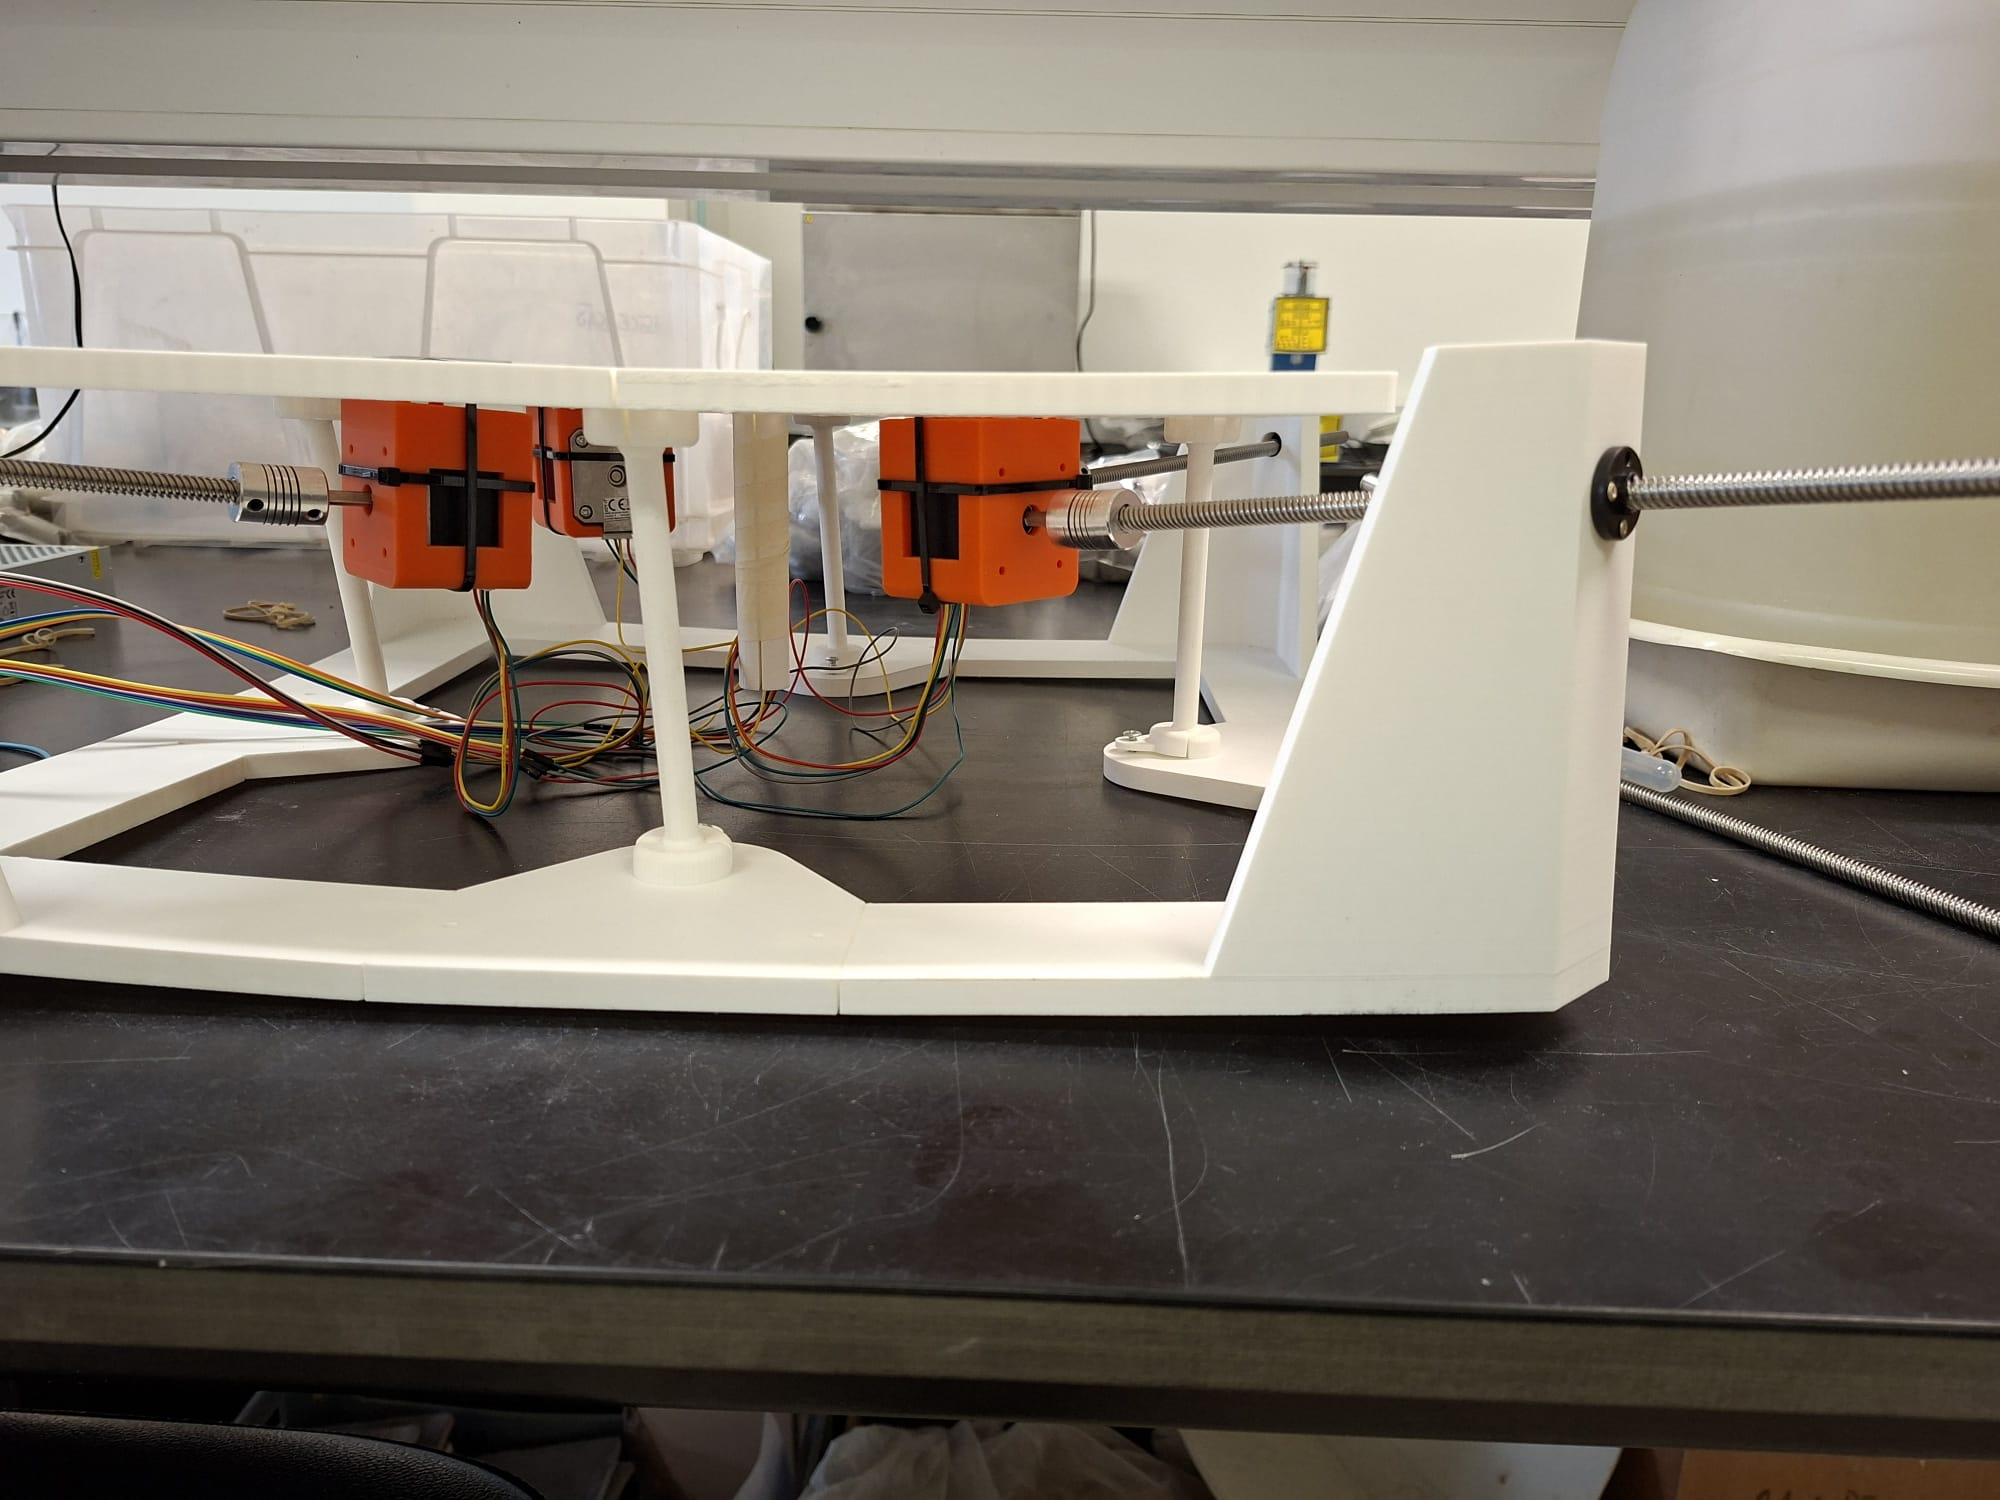
\includegraphics[width=0.75\textwidth]{figs/prototipo_torto.jpeg}
    \caption{Deformação plástica visível na base da mesa após ensaios: o PLA deforma sob a tentativa de replicação sísmica, evidenciando a inadequação do material para solicitações dinâmicas repetidas.}
    \label{fig:prototipo_torto}
\end{figure}

A deformação observada na figura~\ref{fig:prototipo_torto} não é causada por erros de software, pelo que ao ativar os motores eixo a eixo (NS ou EW) não se verificaram estas deformações, mas ao longo da simulação quando o motor não consegue executar todos os passos, o erro acumula e a mesa acaba por deformar.

O efeito combinado destes fatores é que, ao tentar reproduzir o sismo de El Centro à escala real, os motores perdem passo nos picos de velocidade, a plataforma não acompanha o perfil pretendido e a sequência sísmica executada diverge do registo original de forma não controlada.


\subsection{Estratégias Tentadas e Porque Não Resolvem o Problema}
\label{subsec:estrategias-falhadas}

As três estratégias de adaptação do sinal descritas no Capítulo~\ref{chapter:software} foram aplicadas para tentar viabilizar a reprodução sísmica. Nenhuma resolve o problema de fundo:

\begin{itemize}
    \item \textbf{Fator de ajuste ($f_{\text{ajuste}} < 1$):} Com $f_{\text{ajuste}}$ suficientemente baixo, os motores conseguem acompanhar o perfil sem perda de passo - mas devido a como o \textit{firmware} do ESP está feito o motor vai andar a uma aceleração para fazer teóricamente os passos numa determinada janela temporal, ao diminuir os passos e manter a janela o sismo fica muito lento, ao acompanhar a janela voltamos a ter acelerações inantigíveis pelos motores.

    \item \textbf{Clamping (\texttt{max\_steps\_per\_window}):} Limita os picos de velocidade, tornando o perfil executável - mas distorce o conteúdo em frequência do sismo, eliminando precisamente os picos de alta energia que são os mais relevantes para a resposta estrutural. E tal como explicado no ponto acima ao fazer essa redução perdemos velocidade.

    \item \textbf{Subsampling:} Reproduz o sismo em câmara lenta (por exemplo, a 1/4 da velocidade real). Os motores conseguem acompanhar - mas um sismo reproduzido 4$\times$ mais lento não é um sismo: as frequências de excitação descem para fora da gama de ressonância típica de estruturas, o ensaio perde validade sísmica e os resultados não são comparáveis com os de outros estudos experimentais.
\end{itemize}

\textbf{Conclusão:} Nenhuma das estratégias resolve o problema. Para reproduzir fielmente um sismo real à escala temporal correta, seria necessário aumentar o torque disponível (motores NEMA23, alimentação a 24\,V), reduzir o atrito das rótulas (rolamentos, guias lineares). Estas melhorias são detalhadas no Capítulo~\ref{chapter:conclusions}.
